\section{DRAM}
\begin{itemize}
  \item Needs refreshing periodically (every 2-4ms) as capacitor stores data and they lose their charge. Refreshing $\longrightarrow$ read/write/Internal ( hidden refresh, transparent refresh/ cycle stealing).
  \item DRAM's internal organization contains a series of rows and columns. A 256K x 1 DRAM has 25 columns, each containing 256 bits, or eow organized into four section of 64 bits each.

\end{itemize}
\begin{figure}[h!]
  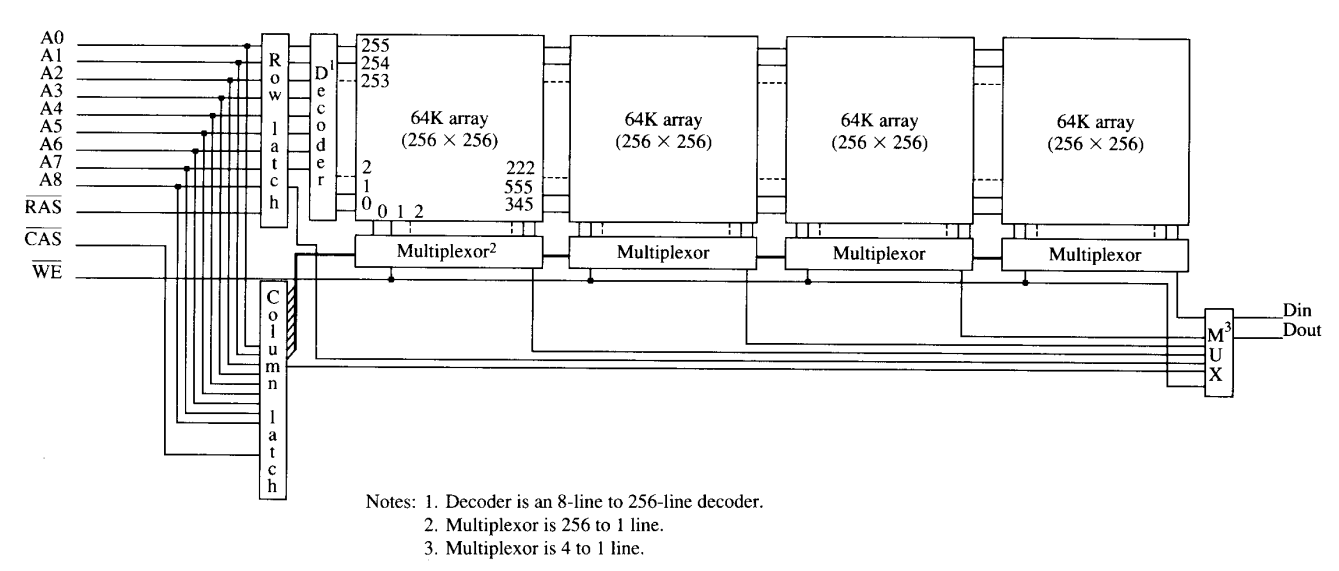
\includegraphics[width = 0.8\textwidth]{./figures/DRAM2.png}
  \caption{The internal structure of a 256K x 1 DRAM. Note that each of the internal 256 words are 1024 bits wide.}
  \label{}
\end{figure}
\begin{itemize}
  \item For refreshing 256 rows in 4ms, refresh cycle is 15.6 $\mu s$
  \item For 8086/8088(for example), clock rate is 5 MHz with 00ns for rd/wr.
\end{itemize}

So, 1 rd/wr$\approx$ 800 ns and 1 refresh cycle $\approx$ 1.5 $\mu s$ \newline
So, 1 refresh cycle $\approx$ $\frac{15.6 \mu s}{800 ns} = 19 rd/wr$ \newline
So, log of 5\%($\approx \frac{1}{19}$) compared to computer time, this is a small price.

\section{EDO memory (Extended  Data Output)}
\begin{itemize}
  \item A slight modification of DRA, where for any memory access, (including a refresh), stores the 25 bits selected by $\overline{RAS}$ into latched.
  \item The latches hold the next 256 bits of information, so that data becomes available without wait in case of sequential execution
  \item Increases system performance by 15-25\%
\end{itemize}

\section{SDRAM (Synchronous Dynamic RAM)}
\begin{itemize}
  \item At the beginning of rd/wr, it behaves like a standard RAM with the same number of wait states.
  \item Subsequent (second, third, and fourth) accesses need 1c.c. each
  \item Therefore to read 4 64-bit numbers, a total of 3(for $1^st$ access) + 1 + 1 + 1 (for next 3 accesses) = 6 cc. are required. For DRAM, it is $3+3+3+3=12 cc.$
  \item 10\% performance increase over EDO.
\end{itemize}

\section{DRAM controllers}
\begin{itemize}
  \item Performs address multiplexing and generation of DRAM control signals
  \item \textbf{Example}: 82C08 - Contains an address multiplexer to mmultiplex a 1-bit address onto 9-bit address connections for 256K memory. It generates $\overline{CAS}$ and $\overline{RAS}$ for DRAM. These signals are developed internally by CLK,$\overline{S_1}$ and $\overline{S_2}$. It takes $\overline{S_1}$ and $\overline{S_0}$ as its $\overline{RD}$ or $\overline{WR}$ inputs. the $\overline{AACK}$/$\overline{XACK}$ provides an acknowledgement output that is used to indicate ready condition of the $\mu P$ (normally connected to READY of $\mu P$)
\end{itemize}
\textbf{Example}: 82C08 connected to a series of four 256K x 8 bit memory composing 1M
\begin{figure}[h!]
  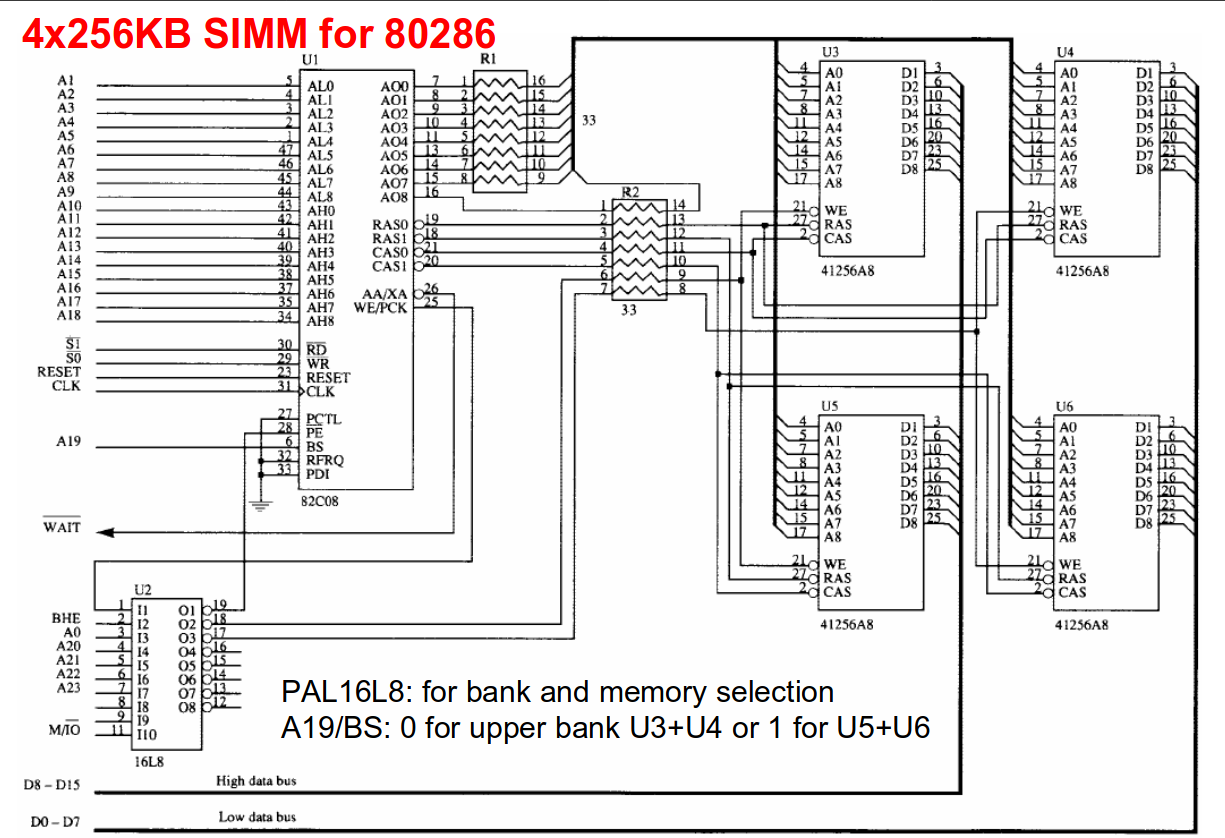
\includegraphics[width = 0.8\textwidth]{./figures/82C08.png}
  \caption{A 1M-byte memory system using four 256K SIMM memory devices and the 82C08 DRAM controller. This section of memory is decoded at locations 000000H-0FFFFFH by the PAL 1L8}
  \label{}
\end{figure}

\begin{itemize}
  \item 82C08 is connected to a series of four 256K x 8 bit memory
  \item U3 and U5 form the high bank, and U4 and U form the low bank.
  \item PAL 16L8 combines $\overline{WE}$ and $A_0$ to generate write signals for U4 and U6 and
  combines $\overline{WE}$ and $\overline{BHE}$ to generate write signals for U3 and U5
  \item PAL also develops the controller selection signal($\overline{PE}$) by combining $M/\overline{IO}$ and other address lines A20-A23
  \item Memory locations 000000H-00FFFFFH\item A19 selects the upper bank (U3 and U4) or the lower bank through the BS (Bank Select)input to 82C08.
  \item PAL logic:
  \begin{enumerate}
    \item $\overline{HWR} = \overline{BHE} \cdot \overline{WE}$
    \item $\overline{LWR} = \overline{A_0} \cdot \overline{WE}$
    \item $\overline{PE} = \overline{A20} \cdot \overline{A21} \cdot \overline{A23} \cdot MIO $
  \end{enumerate}
\end{itemize}
